\section{Results}

\subsection{Held-Out Trajectory Quality}

LatticeFlow reduces selected cost from 3.1415 for direct lattice regression to 2.8805, an 8.31\% decrease (Table~\ref{tab:offline}, Fig.~\ref{fig:offline}). The paired query-level difference is $-0.2610$ with a descriptive 95\% interval of $[-0.2728,-0.2496]$. The decrease appears on both maps: 2.8566 versus 3.1046 on map 8 and 2.9044 versus 3.1783 on map 9.

Mean projected clearance increases from 1.989 to 3.042~m, while the collision proxy decreases from 28.48\% to 18.49\%. Perturbation switching decreases from 4.51\% to 3.38\%, and endpoint shift decreases from 0.1161 to 0.1067~m. These results show that privileged-cost self-improvement can train the complete policy without a pretrained backbone or teacher proposals.

\begin{table}[t]
\caption{Held-out maps 8--9. T: teacher-guided diagnostic. Lower is better except clearance.}
\label{tab:offline}
\centering
\small
\resizebox{\columnwidth}{!}{%
\begin{tabular}{lcccc}
\toprule
Metric & Direct & Residual-T & Physical-T & Ours\\
\midrule
Selected cost & 3.1415 & 2.8622 & \textbf{2.8611} & 2.8805\\
Oracle cost & 2.7946 & \textbf{2.7565} & 2.7629 & 2.7736\\
Clearance (m) & 1.9894 & \textbf{3.1433} & 3.0385 & 3.0421\\
Collision proxy & 28.48\% & \textbf{18.15\%} & 18.90\% & 18.49\%\\
Perturbation switch & 4.51\% & 3.38\% & \textbf{3.22\%} & 3.38\%\\
Endpoint shift (m) & 0.1161 & 0.1011 & \textbf{0.0941} & 0.1067\\
Selection regret & 0.3469 & 0.1057 & \textbf{0.0983} & 0.1069\\
\bottomrule
\end{tabular}}
\end{table}

Teacher information yields a small cost advantage but is not required for the principal gain. Relative to physical-coordinate teacher guidance, the teacher-free selected cost is 0.0193 higher (descriptive 95\% interval $[0.0156,0.0231]$), whereas its collision proxy is 0.41 percentage points lower. Clearance is nearly unchanged, but endpoint shift and regret are 0.0126~m and 0.0086 higher. Late in training, detached student proposals dominate the selected target seeds and accepted gradient steps continue to lower cost, consistent with self-improvement rather than fixed imitation. Only one training seed was evaluated.

Four to six NFE capture nearly all of the flow gain. Selected cost is 2.9519, 2.8916, 2.8823, 2.8805, and 2.8805 for 1, 2, 4, 6, and 8 NFE. Corresponding RTX 5070 Ti full-network latency is 1.540, 1.645, 2.014, 2.616, and 2.646~ms per batch of 16. Thus four NFE increases cost by only 0.065\% relative to six.

\subsection{Closed-Loop Continuity}

Every reported ROS configuration reaches all five goals without geometric collision (Table~\ref{tab:ros}). Raw LatticeFlow is fastest at 8.81~s but exhibits a 0.145 cell-switch rate, confirming that deterministic within-cell flow does not ensure temporal mode consistency. The optional selector reduces switching to 0.024, endpoint jump from 0.271 to 0.164~m, and jerk from 6.45 to 5.56~m/s$^3$, with mean arrival time increasing to 9.62~s. A teacher-guided residual diagnostic remains smoother in endpoint jump and jerk, so the proposed teacher-free model does not dominate every continuity metric.

\begin{table}[t]
\caption{Matched ROS trials on one forest, five goals per configuration.}
\label{tab:ros}
\centering
\small
\resizebox{\columnwidth}{!}{%
\begin{tabular}{lcccccc}
\toprule
Method & Succ. & Time & Switch & Jump & Jerk & Net\\
 &  & (s) &  & (m) & (m/s$^3$) & (ms)\\
\midrule
Direct raw & 5/5 & 9.48 & 0.144 & 0.239 & 6.10 & \textbf{1.17}\\
Residual-T + sel. & 5/5 & 9.73 & 0.026 & \textbf{0.152} & \textbf{4.72} & 2.18\\
Physical-T + sel. & 5/5 & 9.67 & 0.028 & 0.164 & 5.28 & 3.25\\
Ours raw & 5/5 & \textbf{8.81} & 0.145 & 0.271 & 6.45 & 3.26\\
Ours + sel. & 5/5 & 9.62 & \textbf{0.024} & 0.164 & 5.56 & 3.24\\
\bottomrule
\end{tabular}}
\end{table}

\subsection{Perception Alignment and Real Flight}

Sensor-domain matching is necessary for this deployment. On the same 20,000 sparse MID-360 held-out inputs, the standard-view model obtains 5.1706 selected cost and 57.25\% collision proxy; native-FOV training with recorded return masks improves them to 2.9169 and 13.43\%. On 120 recorded real depth frames with a level 4-m goal, the mean complete-trajectory vertical envelope decreases from 0.583 to 0.112~m, and frames within $\pm0.3$~m increase from 0/120 to 120/120.

Removing the virtual ceiling during training does not materially change matched-domain held-out cost (2.9200 without ceiling versus 2.9170 with ceiling), but adding the ceiling only at inference increases cost to 3.2923 and produces upward excursions above 0.3~m in 96.7\% of the recorded frames. The relevant conclusion is train--deployment perception consistency, not that a virtual ceiling is universally beneficial.

\begin{figure*}[t]
    \centering
    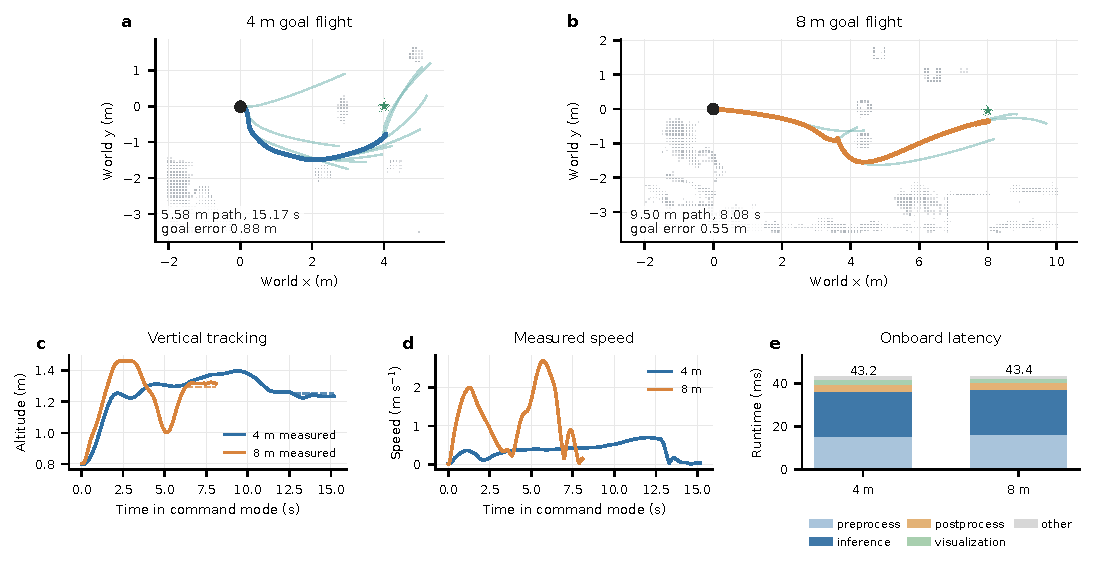
\includegraphics[width=\textwidth]{figures/fig3_real_flights.pdf}
    \caption{LiDAR-only real-flight evidence. (a,b) Complete measured paths, sampled planned trajectories, goals, and accumulated voxelized LiDAR returns for 4-m and 8-m commands. (c) Measured and commanded altitude. (d) Measured speed. (e) Mean onboard timing decomposition. Both flights used TensorRT, six NFE, and raw lattice selection.}
    \label{fig:real}
\end{figure*}

Both real flights complete collision-free obstacle avoidance and enter the 1-m goal region (Fig.~\ref{fig:real}, Table~\ref{tab:real}). The 4-m trial follows a 5.58-m path in 15.17~s and ends 0.88~m from its goal. The 8-m trial follows a 9.50-m path in 8.08~s, ends 0.55~m from its goal, and reaches 2.68~m/s. Altitude remains within 0.798--1.464~m across both trials. Mean inference is 20.8~ms and mean total planning time is 43.3~ms on the Orin NX. These measurements demonstrate onboard feasibility, but two successful flights without a real baseline cannot establish a success rate or comparative safety advantage.

\begin{table*}[t]
\caption{Real-flight bag metrics. Both trials succeeded without observed collision; selector disabled.}
\label{tab:real}
\centering
\small
\resizebox{\textwidth}{!}{%
\begin{tabular}{lrrrrrrrc}
\toprule
Trial & Goal (m) & Duration (s) & Path (m) & $v_{\max}$ (m/s) & Goal error (m) & Altitude (m) & Inference / total (ms) & Outcome\\
\midrule
Flight 1 & 4 & 15.17 & 5.58 & 0.70 & 0.88 & 0.798--1.400 & 21.12 / 43.18 & success\\
Flight 2 & 8 & 8.08 & 9.50 & 2.68 & 0.55 & 0.803--1.464 & 20.50 / 43.39 & success\\
\bottomrule
\end{tabular}}
\end{table*}
